\cia\vspace{-2cm}
\section{Electron Fiducial cuts} 
\label{sec:fid_e} 
A fiducial cut on electrons is introduced to constrain regions of phase space
where the CLAS response peaks at its maximum and remains rather smooth.
The \v Cerenkov detector presents a drop in optical efficiency 
(see \F{fig:optical_drop}) which is not simulated by the MonteCarlo, therefore 
these regions have to be removed. 
\begin{figure}[h]
 \begin{center}
 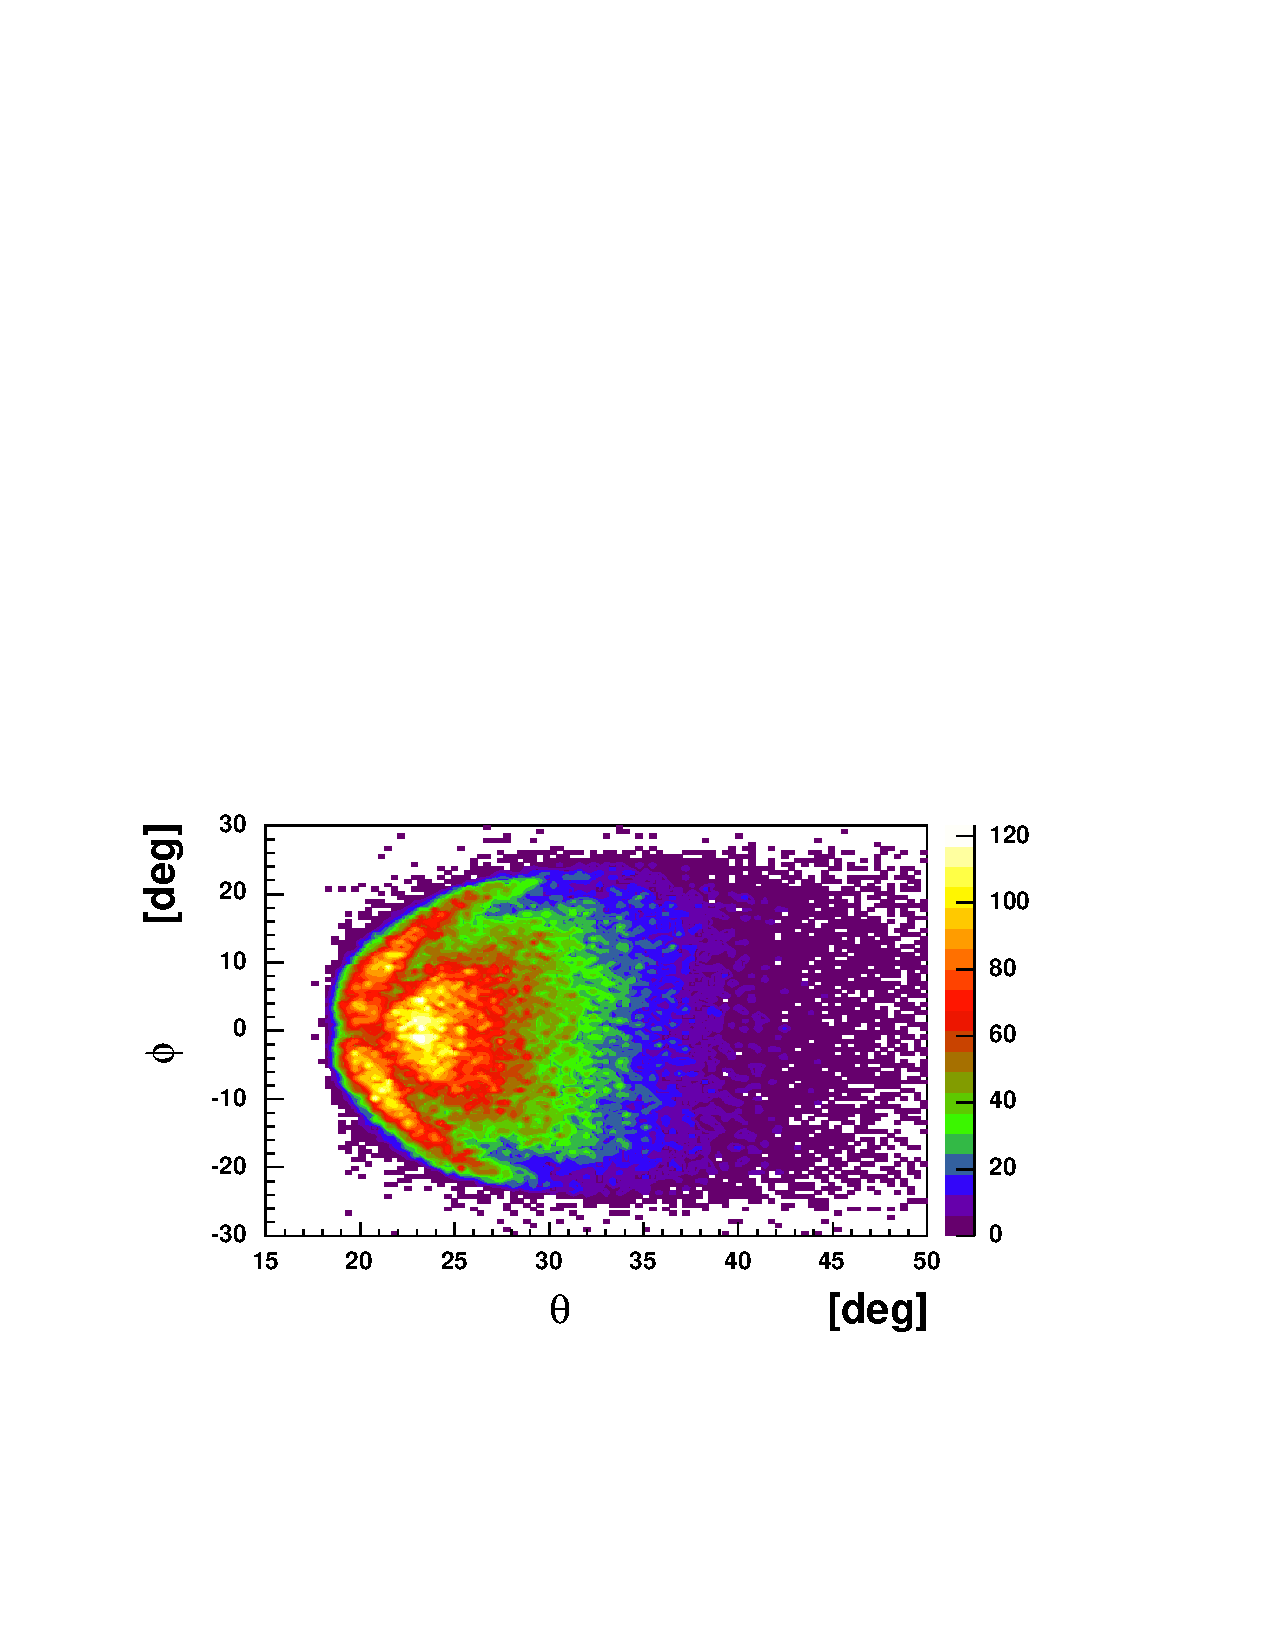
\includegraphics[width = 10cm, bb=100 140 460 440]{data_reduction/img/electron_before_id} 
  \caption[$\phi$ versus $\theta$ for sector 1 electrons before the electron ID]
          { $\phi$ versus $\theta$ for sector 1 electrons before the electron ID. 
                     The electron ID suppress the external bands as shown in \F{fig:fidu_etph}.}
 \label{fig:optical_drop}
 \end{center}
\end{figure}
Drift chamber and time of flight inefficiencies (dead or inefficient wires, dead phototubes)
cause holes and depletions in the acceptance. While most of these symptoms appears in 
the GSIM simulation, some do not\footnote{One reason is that there are switched
wires in the DC not accounted in the simulation.}. 

Furthermore the boundaries of all these regions differ
when comparing actual data and simulation.

\subsection{ $\phi$ boundaries}
For each sector, an empirical cut on $\phi$ is introduced as a function of theta and momentum:
$$ 
 \phi \,\,\le\,\, \Delta\phi \,(\theta, p)
$$
which is aimed to define regions of phase space whose distributions are flat in $\phi$.
After careful study \cite{bib:fid_e}, the mathematical form of the cut depends on 6 parameters  $C_i$
and assumes the form:\vspace{-0.3 cm}
$$
\begin{array}{c c c}
\\
\Delta\phi   & = &  C_4 \left( \sin (\theta - \theta_{cut}) \right) ^{\,E} \\
\\
E        & = &  C_3\, p\, ^{C_5} \\
\\
\theta_{cut} & = &  C_1 + \Dfrac{C_2}{p + C_6}
\end{array}
$$
A $\phi$ vs $\theta$ distribution was plotted for 10 different momentum bins from $1.6$ to $4.6$ GeV.
\F{fig:fidu_etph} shows one example ($p=1.9-2.2$ GeV) of such distributions.
\begin{figure}[h]
 \begin{center}
 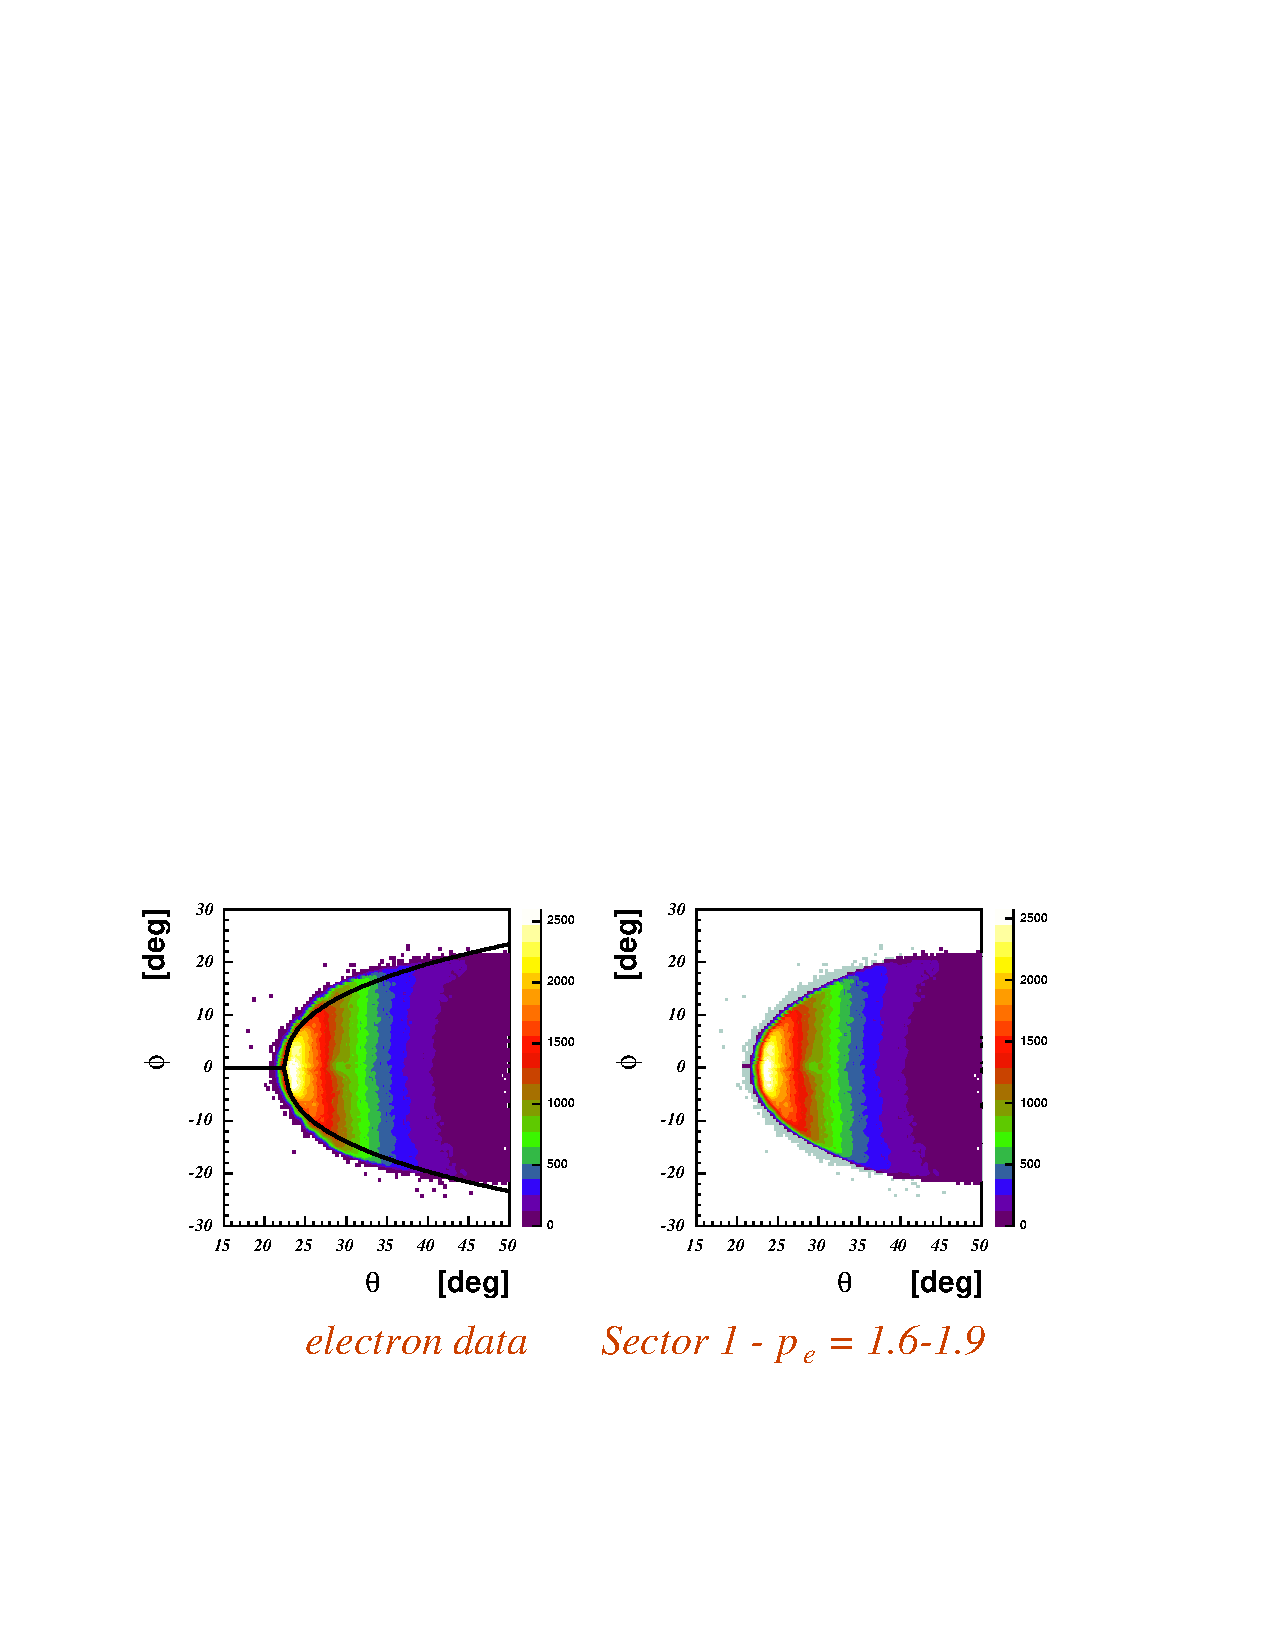
\includegraphics[width = 14cm, bb=0 130 550 400]{data_reduction/img/electron_tph} 
  \caption[$\phi$ versus $\theta$ for sector 1 and $p=1.6-1.9$ GeV]
          { $\phi$ versus $\theta$ for sector 1 and $p=1.6-1.9$ GeV after the electron ID. Left:
                     before fiducial cut. Right: before fiducial cut (box/gray) and after fiducial cut (color contour). 
                     For all the
                     bins in all the sectors, see
                     {\tt  http://www.jlab.org/$\sim$ungaro/pi0eprod/fiducial\_cut\_e}
          }
 \label{fig:fidu_etph}
 \end{center}
\end{figure}
The $\phi$ distributions are also plotted for $\theta$ slices one degree wide as in \F{fig:fidu_ephis}
and the $C_i$ parameters are adjusted empirically.
See    \begin{verbatim} http://www.jlab.org/~ungaro/pi0eprod/fiducial_cut_e/ \end{verbatim}
for all the plots.

\begin{figure}[h]
 \begin{center}
 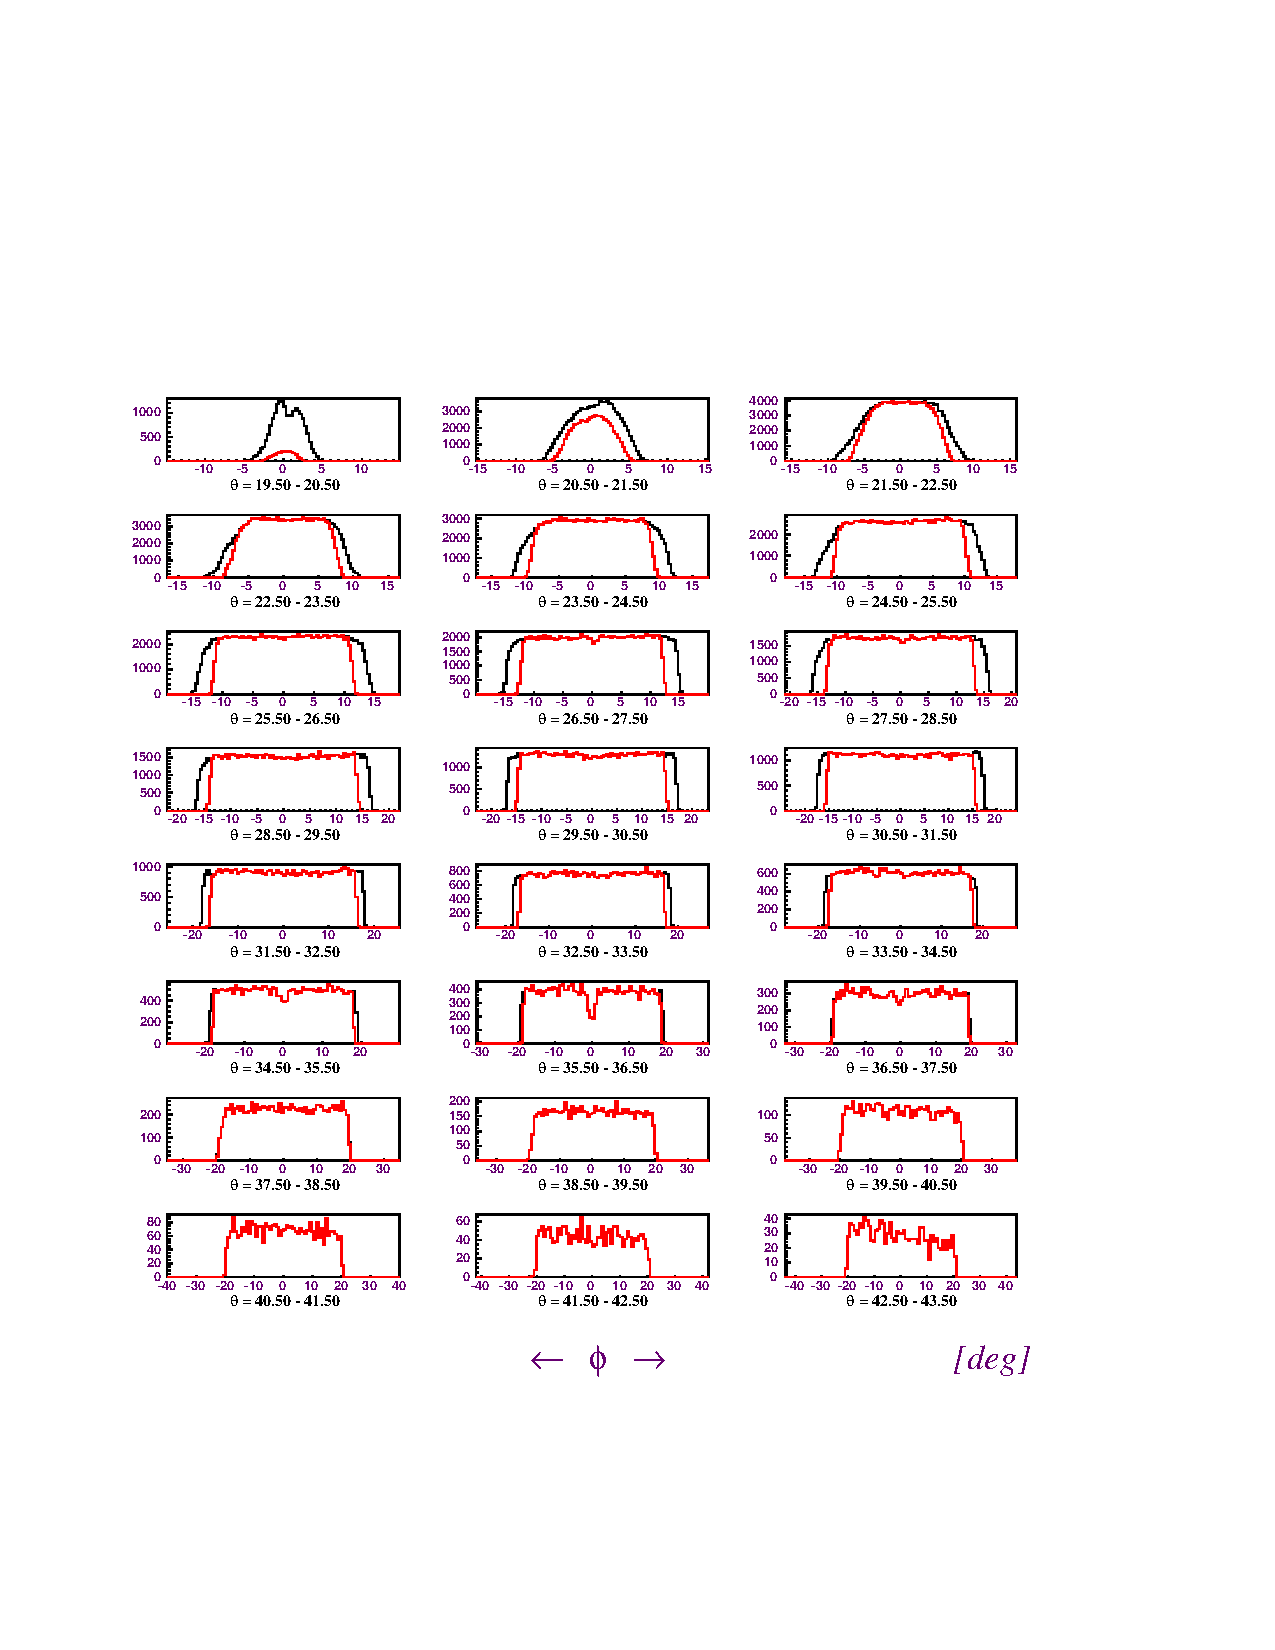
\includegraphics[width = 14cm, bb=60 120 500 610]{data_reduction/img/electron_phis} 
  \caption[$\phi$ distributions (sector 3) for different $\theta$ and $p=1.9-2.2$ GeV]
          { $\phi$ distributions (sector 3) for different $\theta$ and $p=1.9-2.2$ GeV. Black: before fiducial
                     cut. Red: after fiducial cut. 
		     \v Cerenkov inefficiency (section \ref{sec:cc_eff}) is responsible for some irregularities
		     at $\phi = 0$ (for example at  $\theta = 35.5^0 - 36.5^0$) while drift chamber and time of flight
		     inefficiency (section \ref{sec:dc_ineff}) 
		     causes other irregularities (for example at  $\theta = 42.5^0 - 43.5^0$).}
 \label{fig:fidu_ephis}
 \end{center}
\end{figure}
\cia
Table \ref{tab:fid_epars} shows the 6 parameters obtained. \F{fig:fidu_e3d} shows the fiducial cut as a function
of $p$, $\theta$ and $\phi$ for sector 1.
\vspace{1cm}
\begin{table}[h]
 \begin{center}
  \begin{tabular}{|c|c|c|c|c|c|c|}
    \hline 
   Sector & $C_1$ & $C_2$ & $C_3$ & $C_4$     & $C_5$ & $C_6$ \\
    \hline  
   1 &     12.0 &  20.0 &  0.32 &  32.0 &  0.416667 &  0.14 \\
   2 &     //   &  20.7 &  0.36 &  34.0 &  //       &  // \\
   3 &     //   &  20.2 &  0.32 &  32.0 &  //       &  // \\
   4 &     //   &  20.5 &  0.32 &  32.0 &  //       &  // \\
   5 &     //   &  20.5 &  0.29 &  32.0 &  //       &  // \\
   6 &     //   &  20.0 &  0.32 &  32.0 &  //       &  // \\
 \hline
  \end{tabular}
 \end{center} 
 \caption[The 6 parameters for electron fiducial cut for each of the 6 sectors.]
         { The 6 parameters for electron fiducial cut for each of the 6 sectors. 
	            Only $C_2$, $C_3$, $C_4$ are sector dependent. }
 \label{tab:fid_epars}
\end{table}

\begin{figure}[h]
 \begin{center}
 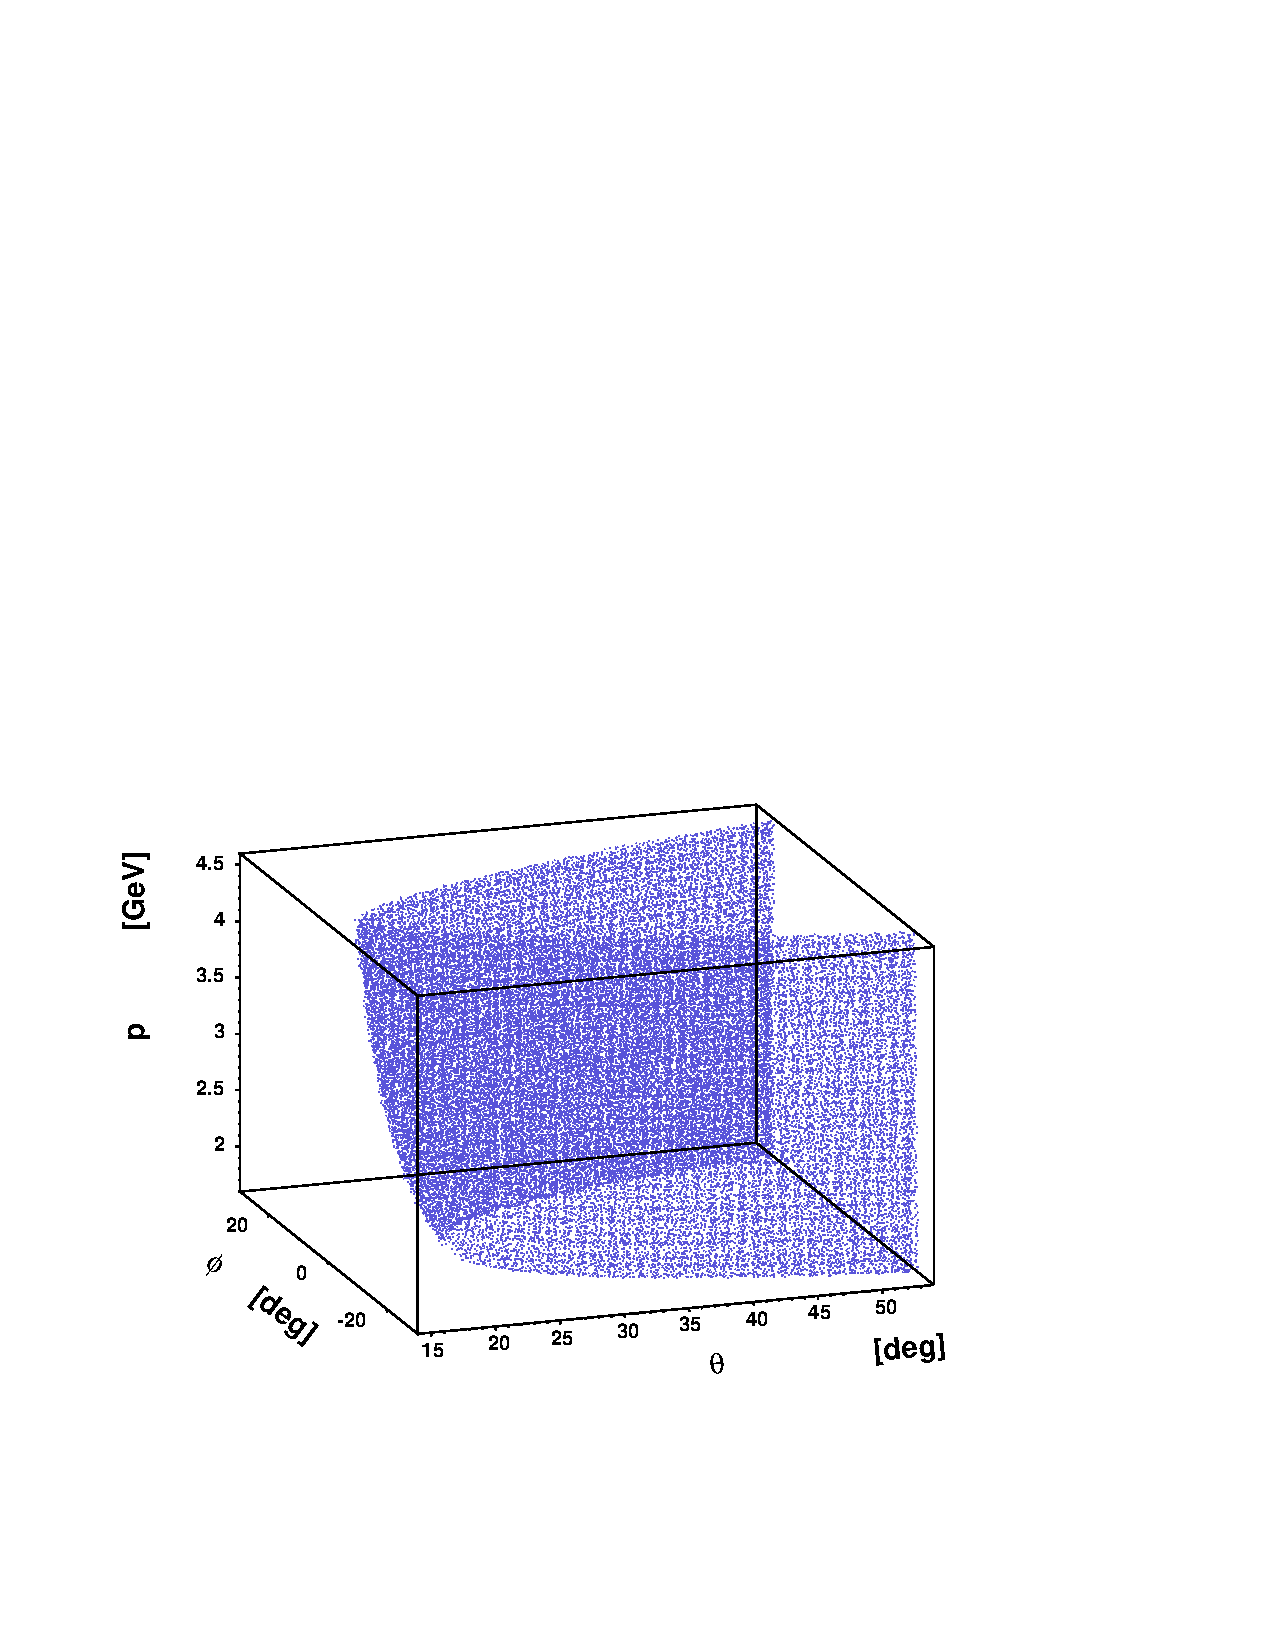
\includegraphics[width = 12cm, bb=20 120 480 480]{data_reduction/img/electron_tphp} 
  \caption[The electron fiducial cut for sector 1]
          { The electron fiducial cut for sector 1. The cut starting point moves back
	             as the momentum increases (and $\theta$ decreases). 
		     This causes the cut to narrow up with momemtum because electrons are detected 
		     near the lower edges of the detectors. }
 \label{fig:fidu_e3d}
 \end{center}
\end{figure}

\cia
\subsection{  $\theta$ versus momentum cuts}
Sector 2, 5 and 6 present holes and depletions (mainly because of dead time of flight paddles) 
which are taken care of with the 
cuts shown in \F{fig:fidu_etp5} where $\theta$ is plotted versus $p$.
\begin{figure}[h]
 \begin{center}
 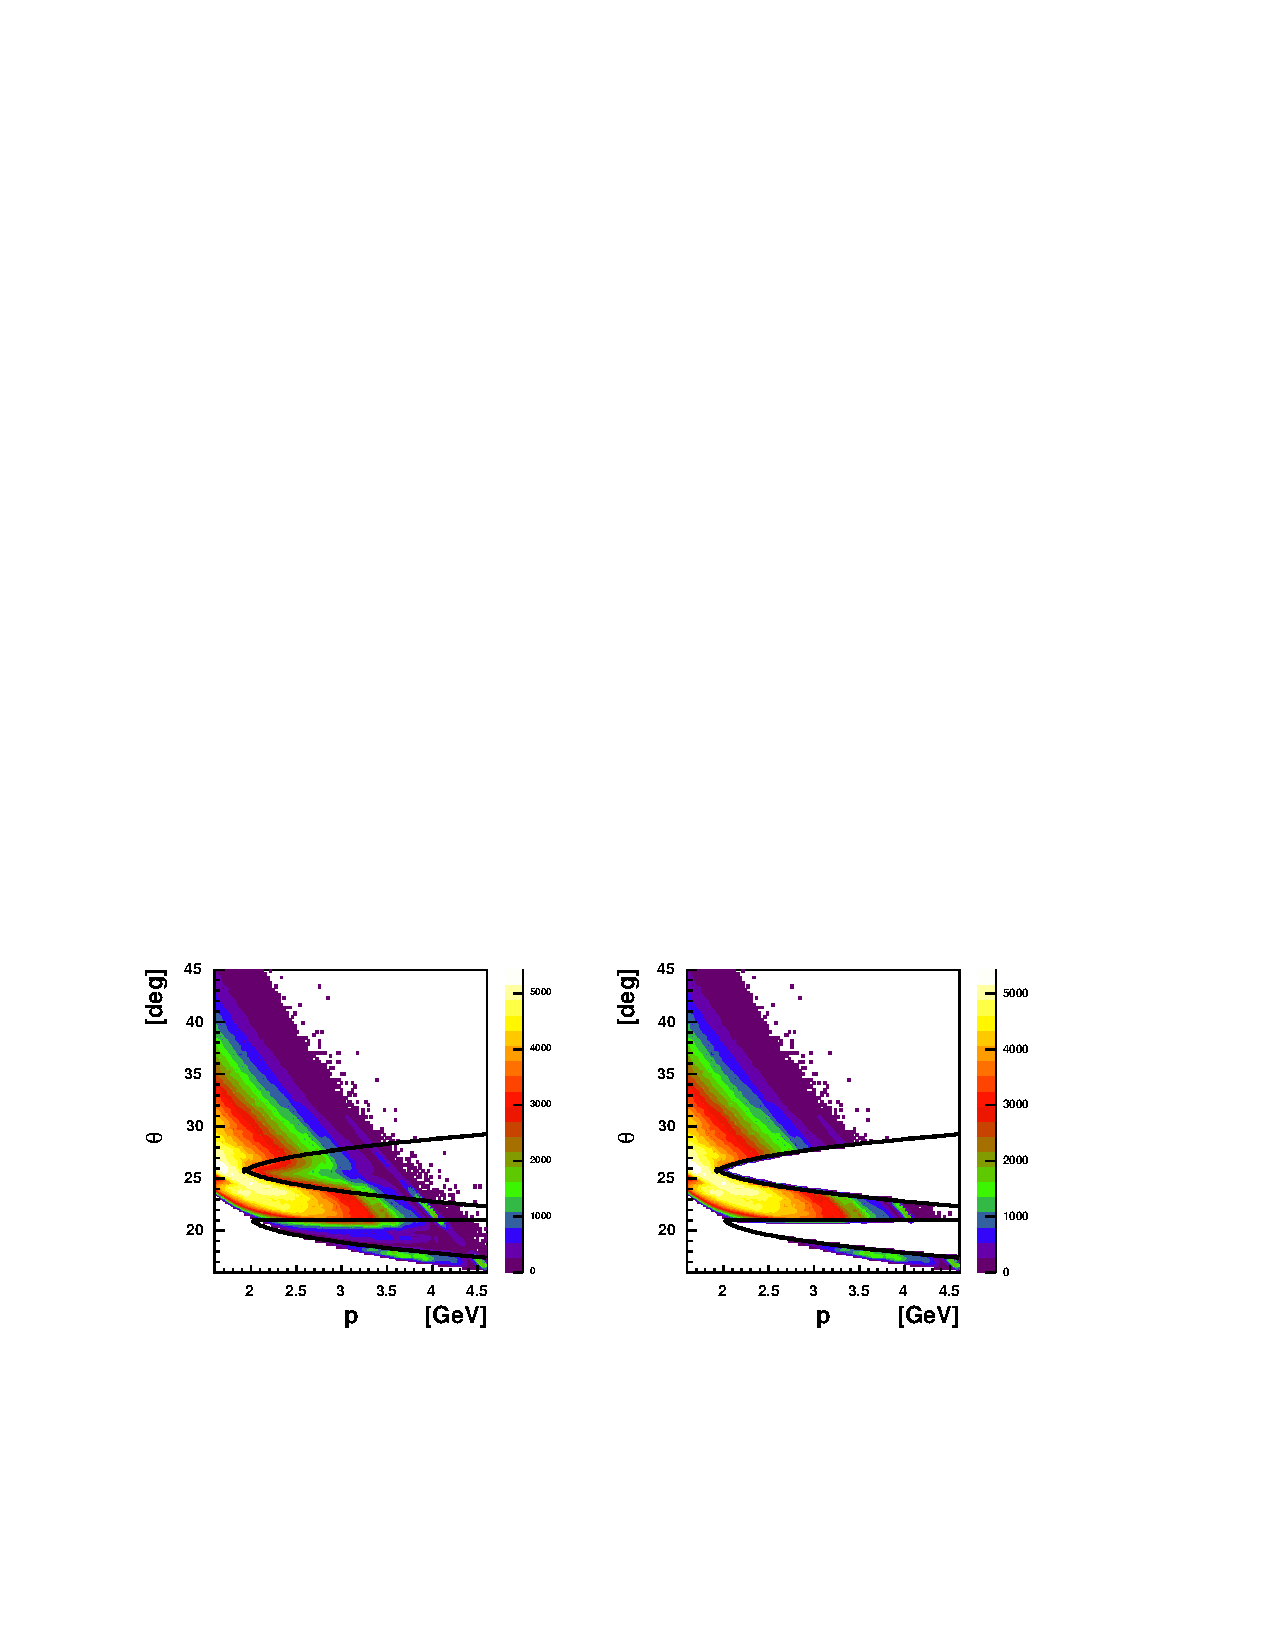
\includegraphics[width = 14cm, bb=60 140 500 380]{data_reduction/img/electron_tp5}  
  \caption[$\theta$ versus $p$ for sector 5]
          { $\theta$ versus $p$ for sector 5. Two depletions are clearly visible and cut out.}
 \label{fig:fidu_etp5}
 \end{center}
\end{figure}
\\
A summary of all the cuts used for the electron fiducial cut can be found in Appendix \ref{app:fidu_e}.
\F{fig:sum_s6} shows the    effects of the fiducial cuts on the $\phi$
versus $\theta$ distribution in sector 6.

\begin{figure}
 \begin{center}
 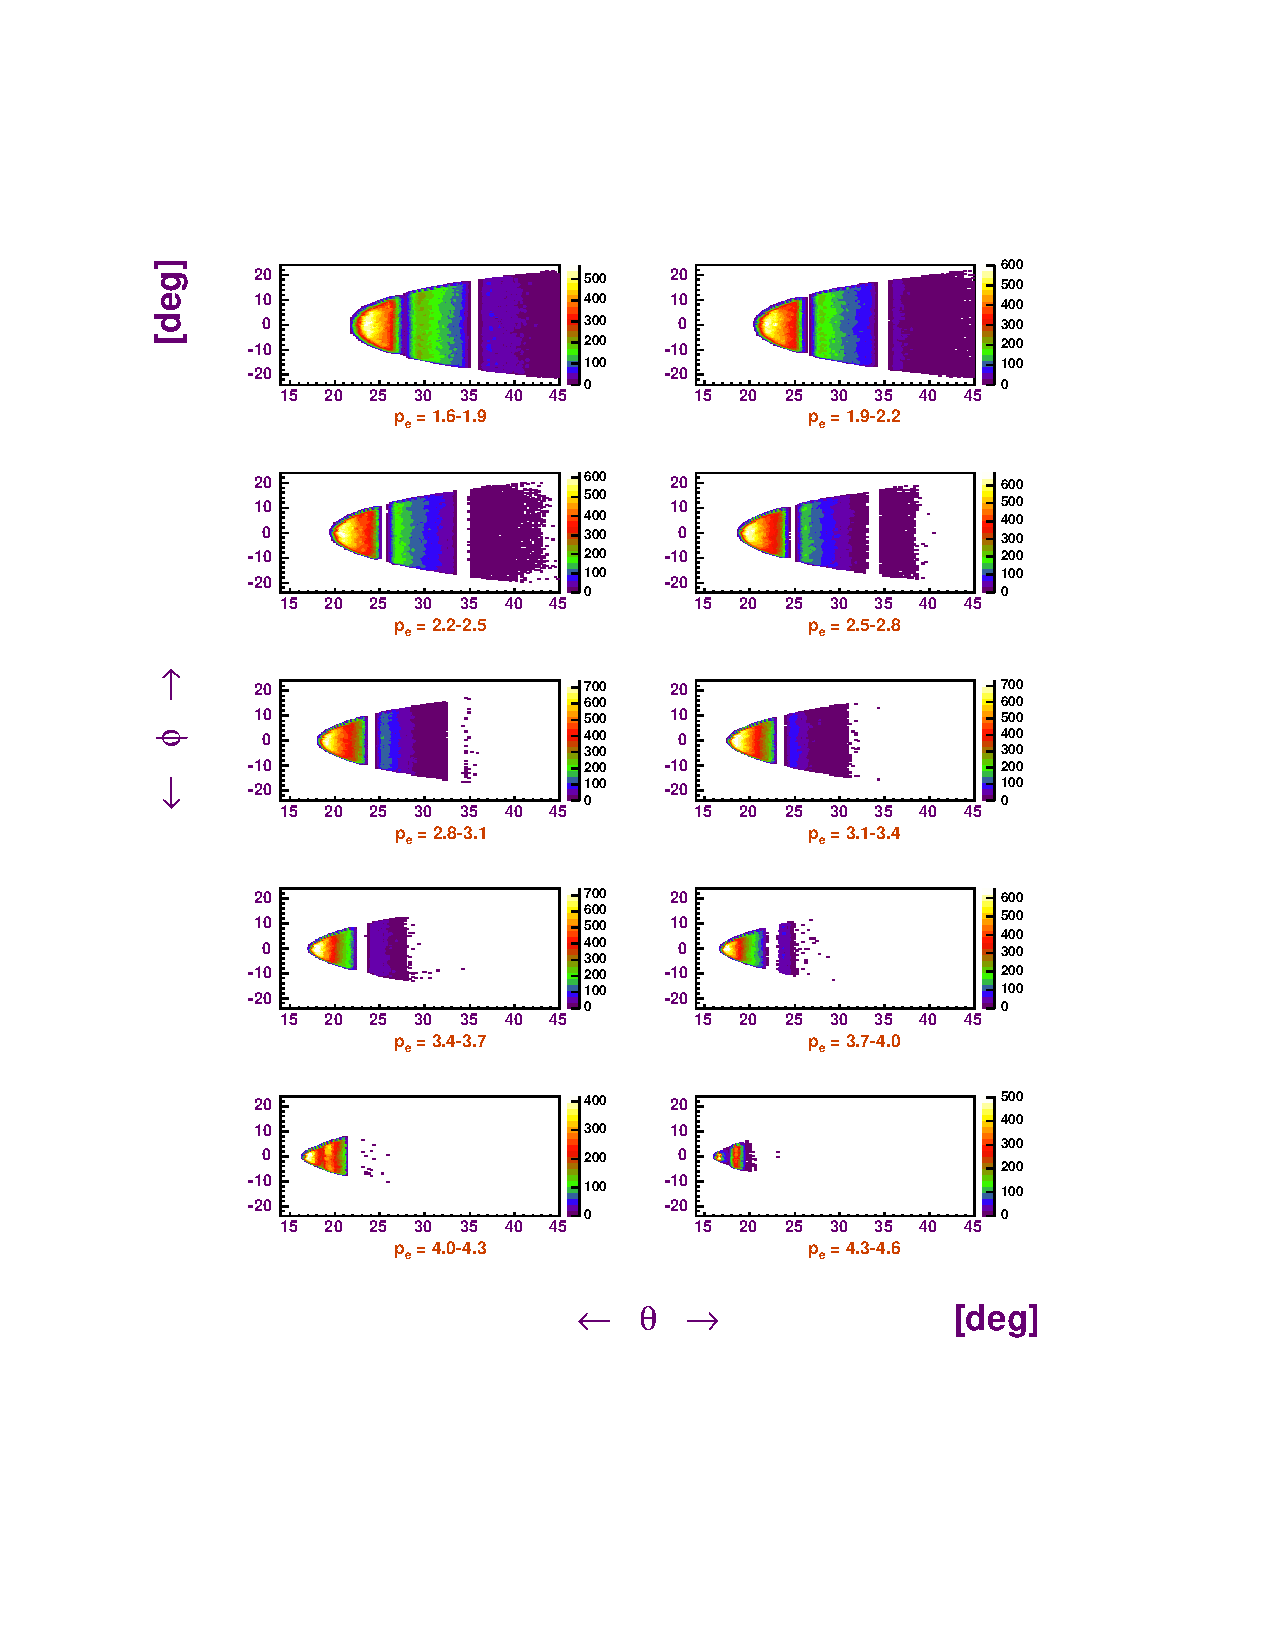
\includegraphics[width = 14cm, bb=60 120 520 700]{data_reduction/img/summary_sec6}  
  \caption[$\phi$ versus $\theta$ distribution for sector 6 after fiducial cuts]
          { $\phi$ versus $\theta$ distribution for sector 6 after fiducial cuts. The $\theta$ versus
                     $p$ cuts are reflected on this plane as vertical bands. }
 \label{fig:sum_s6}
 \end{center}
\end{figure}












